\documentclass[shadesubsections,compress,14pt,mathserif]{beamer}
\usepackage[danish]{babel}	
\usepackage{tikz}
\usetikzlibrary{shapes, positioning}
\usenavigationsymbolstemplate{}
\usepackage{pgfplots}
\usepackage[absolute,overlay]{textpos}

%\usepackage[T1]{fontenc}
%\usepackage{fourier}
% Dokumentets sprog
%\usepackage{mathtools}
%\usepackage{pxfonts}
\usepackage{eulervm}
% Class options include: notes, notesonly, handout, trans,
%                        hidesubsections, shadesubsections,
%                        inrow, blue, red, grey, brown

% Theme for beamer presentation.
%\usepackage{beamertheme} 
% Other themes include: beamerthemebars, beamerthemelined, 
%                       beamerthemetree, beamerthemetreebars  
 \newcommand{\prot}{\mathbf{P}}
\newcommand{\adv}{\ensuremath{\mathcal A}}
\newcommand{\aggdeg}[1]{\mathfrak{d}(#1)}
\renewcommand{\deg}{\mathrm{deg}}
\newcommand{\xor}{\ensuremath{\oplus}}
\newcommand{\plonk}{\ensuremath{\mathcal{P} \mathfrak{lon}\mathcal{K}}}
\newcommand{\F}{\ensuremath{\mathbb F}}
\newcommand{\set}[1]{\ensuremath{\left\{#1\right\}}}
\newcommand{\sett}[2]{\ensuremath{\left\{#1\right\}_{#2}}}
\newcommand{\enc}[1]{\ensuremath{\left[#1\right ]}}
\newcommand{\cm}{\ensuremath{\mathsf{cm}}}
\newcommand{\open}[1]{\ensuremath{\mathsf{open}(#1)}}
\newcommand{\verify}[1]{\ensuremath{\mathsf{verify}(#1)}}
\newcommand{\defeq}{\ensuremath{:=}}
\newcommand{\helper}{\ensuremath{\mathcal{H}}}
\newcommand{\ver}{\ensuremath{\mathcal{V}}}
\newcommand{\prv}{\ensuremath{\mathcal{P}}}
 \newcommand{\polysofdeg}[1]{\F_{< #1}[X]}
 \newcommand{\polys}{\F[X]}
\newcommand{\acc}{{\mathbf{acc}}}
\newcommand{\ideal}{\mathbf{I}}
\newcommand{\gen}{\alpha}
\newcommand{\plookup}{\mathsf{plookup}}
%\setbeamersize{text margin left=3mm,text margin right=3mm} 
\title{\large{Ranged Polynomial Protocols}}    % Enter your title between curly braces
\author{\small{Ariel Gabizon}\\                 % Enter your name between curly braces
\tt{\footnotesize{\textbf{Aztec}\\ (Based on work with Zachary J. Williamson)                                        } }      }% Enter your institute name between curly braces
\date{}                    % Enter the date or \today between curly braces
%\usefonttheme{professionalfonts}
%\usefonttheme[onlymath]{serif}
\begin{document}
\boldmath
% Creates title page of slide show using above information
\begin{frame}
  \titlepage
\end{frame}



\begin{frame}
% \frametitle{The trusted setup sliding scale (until 2018)}   % Insert frame title between curly braces
 \begingroup
 \centering
 
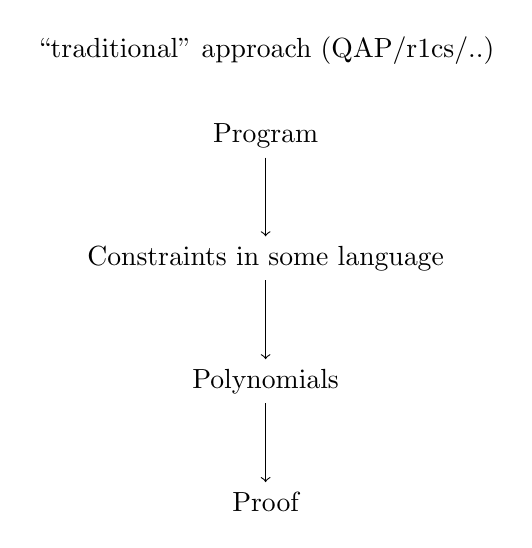
\begin{tikzpicture}[ball/.style={circle, minimum width=1cm, minimum height=1cm, draw}]
% \node[ball] (gate1) {+};
% \node[ball, above right=1.25cm of gate1] (gate2) {$\times$};
\node[]  (text0) {``traditional'' approach (QAP/r1cs/..)};
\node[below = 0.5cm of text0]  (text1) {Program};
\node[below=1cm of text1] (text2){Constraints in some language};
% \node[below=2cm of text1] (text2) {universal updatable setup  (our choice)};
\node[ below=1cm of text2] (text3) {Polynomials};   
\node[ below=1cm of text3] (text4) {Proof};   


\draw[->] (text1) -- (text2);
\draw[->] (text2) -- (text3);
\draw[->] (text3) -- (text4);

\end{tikzpicture}
% This talk (\small{similar in spirit to [..,BCGGHJ17,Arya,..]}):
% \begin{tikzpicture}[ball/.style={circle, minimum width=1cm, minimum height=1cm, draw}]
% % \node[ball] (gate1) {+};
% % \node[ball, above right=1.25cm of gate1] (gate2) {$\times$};
% \node[]  (text1) at (5,100) {Program};
% % \node[below=2cm of text1] (text2) {universal updatable setup  (our choice)};
% \node[ right=1cm of text1] (text2) {Thing with polynomials};   
% \node[ right=1cm of text2] (text3) {proof};   
% 
% 
% \draw[->] (text1) -- (text3);
% 
% \end{tikzpicture}

 \endgroup
 
\end{frame}
\begin{frame}
% \frametitle{The trusted setup sliding scale (until 2018)}   % Insert frame title between curly braces
 \begingroup
 \centering
 
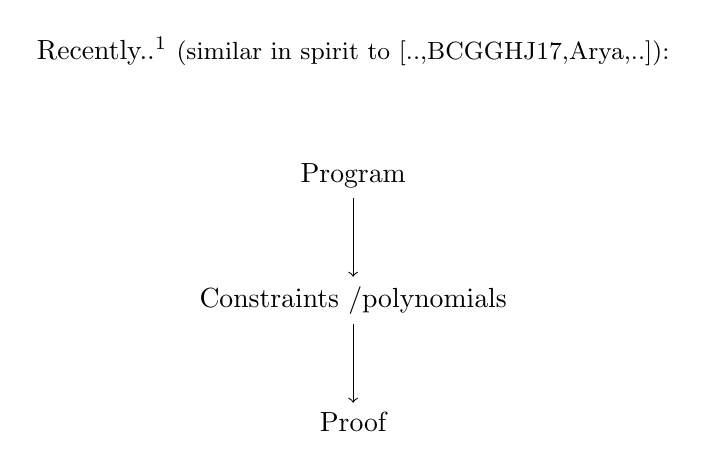
\begin{tikzpicture}[ball/.style={circle, minimum width=1cm, minimum height=1cm, draw}]
% \node[ball] (gate1) {+};
% \node[ball, above right=1.25cm of gate1] (gate2) {$\times$};
% \node[]  (text0) {``traditional'' approach (QAP/r1cs/..)};
% \node[below = 0.5cm of text0]  (text1) {Program};
% \node[below=1cm of text1] (text2){Constraints in some language};
% % \node[below=2cm of text1] (text2) {universal updatable setup  (our choice)};
% \node[ below=1cm of text2] (text3) {Thing with polynomials};   
% \node[ below=1cm of text3] (text4) {Proof};   
% 
% 
% \draw[->] (text1) -- (text2);
% \draw[->] (text2) -- (text3);
% \draw[->] (text3) -- (text4);
% 
% \node[ball] (gate1) {+};
% \node[ball, above right=1.25cm of gate1] (gate2) {$\times$};
\node[]  (text5) { Recently..\footnote{https://ethresear.ch/t/using-polynomial-commitments-to-replace-state-roots/7095,$\plookup$}  \small{(similar in spirit to [..,BCGGHJ17,Arya,..])}:};
\node[below = 1cm of text5]  (text6) {Program};
% \node[below=1cm of text6] (text7){};
% \node[below=2cm of text1] (text2) {universal updatable setup  (our choice)};
\node[ below=1cm of text6] (text7) {Constraints /polynomials};   
\node[ below=1cm of text7] (text8) {Proof};   


\draw[->] (text6) -- (text7);
\draw[->] (text7) -- (text8);
% \draw[->] (text3) -- (text4);

\end{tikzpicture}
% 
% \end{tikzpicture}

 \endgroup
 
\end{frame}

% 
% \begin{frame}
% \frametitle{Idealized Polynomials Protocols}   % Insert frame title between curly braces
% %Since the beginning of time (LFKN, 1989) humanity has been trying to verify prover polynomial evaluations.\\
%  
%  \textbf{Preprocessing:} $\ver$ chooses polynomials $g_1,\ldots,g_t\in \polysofdeg{d}$.\\
%  \vspace{0.4in}
% \textbf{Protocol:}
%   \begin{enumerate}
% %\item The protocol definition includes a set of \emph{preprocessed polynomials} $g_1,\ldots,g_\ell \in \polysofdeg{d}$.
% 
% \item 
% $\prv$'s  msgs are to ideal party $\ideal$. Must be $f_i\in \polysofdeg{d}$.
%  \item At protocol end $\ver$ asks $\ideal$ if some identities hold between $\set{f_1,\ldots,f_\ell,g_1,\ldots,g_t}$.  Outputs $\acc$ iff they do.
% \end{enumerate}
% \end{frame}
% \begin{frame}
% \frametitle{Idealized Polynomials Protocols}   % Insert frame title between curly braces
% %Since the beginning of time (LFKN, 1989) humanity has been trying to verify prover polynomial evaluations.\\
%  
%  \textbf{Preprocessing:} $\ver$ chooses polynomials $g_1,\ldots,g_t\in \polysofdeg{d}$.\\
%  \vspace{0.2in}
% \textbf{Protocol:}
%  
%  \begin{enumerate}
% %\item The protocol definition includes a set of \emph{preprocessed polynomials} $g_1,\ldots,g_\ell \in \polysofdeg{d}$.
% 
% \item $\prv$'s  msgs are to ideal party $\ideal$. Must be $f_i\in \polysofdeg{d}$.
% \item At end, $\ver$ asks $\ideal$ if some identities hold between $\set{f_1,\ldots,f_\ell,g_1,\ldots,g_t}$.  
% 
% 
% \end{enumerate}
% \emph{Using [KZG10], can compile to real protocol with each msg of $\prv$ being 32-48} 
% 
% \end{frame}
% 

% \begin{frame}
% \textbf{Feel life is too short to constantly cite the fundamental thm of Algebra?}
% \end{frame}

% \begin{frame}
% \frametitle{$H$-ranged Polynomials Protocols}   % Insert frame title between curly braces
% %Since the beginning of time (LFKN, 1989) humanity has been trying to verify prover polynomial evaluations.\\
%  
%  \textbf{Preprocessing:} $\ver$ chooses polynomials $g_1,\ldots,g_t\in \polysofdeg{d}$, $H\subset\F$.\\
%  \vspace{0.4in}
% \textbf{Protocol:}
%  
%  \begin{enumerate}
% %\item The protocol definition includes a set of \emph{preprocessed polynomials} $g_1,\ldots,g_\ell \in \polysofdeg{d}$.
% 
% \item $\prv$'s  msgs are to ideal party $\ideal$. Must be $f_i\in \polysofdeg{d}$.
% \item At end, $\ver$ asks $\ideal$ if some identities hold between $\set{f_1,\ldots,f_\ell,g_1,\ldots,g_t}$   \textbf{\textit{on $H$}}. 
% 
% \end{enumerate}
% \end{frame}
\begin{frame}
\frametitle{Ranged polynomials protocols}   % insert frame title between curly braces
%since the beginning of time (lfkn, 1989) humanity has been trying to verify prover polynomial evaluations.\\

\textbf{Preprocessing/inputs:} Predefined polynomials $g_1,\ldots,g_t\in \polysofdeg{d}$\\
\textbf{Range:} $H\subset\F$.\\ \pause
\vspace{0.4in}
\textbf{Protocol:}
 
 \begin{enumerate}
%\item The protocol definition includes a set of \emph{preprocessed polynomials} $g_1,\ldots,g_\ell \in \polysofdeg{d}$.

\item $\prv$'s  msgs are to ideal party $\ideal$. Must be $f_i\in \polysofdeg{d}$.\pause
\item At end, $\ver$ asks $\ideal$ if some identity holds between $\set{f_1,\ldots,f_\ell,g_1,\ldots,g_t}$   \textbf{\textit{on $H$}}. 

\end{enumerate}
\end{frame}
\begin{frame}
% \frametitle{$h$-ranged polynomials protocols}   % insert frame title between curly braces
%since the beginning of time (lfkn, 1989) humanity has been trying to verify prover polynomial evaluations.\\

$D\defeq$ max degree of identity $C$ checked in exec with honest $\prv$.\\
 \vspace{0.2in}

 $\aggdeg{\prot}\defeq$ $\left(\sum_{i\in [t]} \deg(f_i)+1\right)+D -|H|$.\pause \\
 \vspace{0.2in}
\textbf{Thm:\footnote{similar statements in Marlin/Fractal/Supersonic}}
Can compile to ``real'' protocol in Algebraic Group Model, where prover complexity ~ $\aggdeg{\prot}$ .\\ \pause
 \vspace{0.2in}
\textbf{proof sketch:}
 Use [KZG] polynomial commitment scheme. $\prv$ commits to all polys and $C/Z_H$. $\ver$ checks identity at random challenge point. 
\end{frame}


\begin{frame}
\frametitle{Multiset equality check}
%Since the beginning of time (LFKN, 1989) humanity has been trying to verify prover polynomial evaluations.\\
Given $a,b\in \F^3$, want to check $\{b_1,b_2,b_3\} \stackrel{?}{=} \{a_1,a_2,a_3\}$ \\ \pause
 \vspace{0.2in}

  
 Choose random $\gamma\in \F$. Check
  \[(a_1 + \gamma)(a_2+ \gamma)(a_3 + \gamma) \stackrel{?}{=} (b_1+\gamma)(b_2+\gamma)(b_3+\gamma)\]\pause
%   \[a'_1 = a_1 + \gamma, a'_2 = a_2 + \gamma, a'_3 = a_3 + \gamma\]
%  \[b'_1 = b_1 + \gamma, b'_2 = b_2 + \gamma, b'_3 = b_3 + \gamma\]\pause

 \vspace{0.2in}
 If $a,b$ different as sets then w.h.p products different.\pause
 
\end{frame}



\begin{frame}
\frametitle{Multiset equality check - polynomial version}
%Since the beginning of time (LFKN, 1989) humanity has been trying to verify prover polynomial evaluations.\\
Given $f,g\in \polysofdeg{d}$, want to check $\sett{f(x)}{x\in H} \stackrel{?}{=} \sett{g(x)}{x\in H}$ as multisets \\ 
 
\end{frame}

\begin{frame}
\frametitle{Multiplicative subgroups:}   % Insert frame title between curly braces
%Since the beginning of time (LFKN, 1989) humanity has been trying to verify prover polynomial evaluations.\\
 $H=\set{\gen,\gen^2,\ldots,\gen^n=1}$.\\
 \vspace{0.2in}
 $L_i$ is i'th lagrange poly of $H$:
 \[L_i(\alpha^i)=1,L_i(\alpha^j) =0, j\neq i\]
\end{frame}


\begin{frame}
\frametitle{Reduces to:}   % Insert frame title between curly braces
%Since the beginning of time (LFKN, 1989) humanity has been trying to verify prover polynomial evaluations.\\
 $H=\set{\gen,\gen^2,\ldots,\gen^n}$.\\
 \vspace{0.2in}
 
 $\prv$ has sent $f,g\in \polysofdeg{n}$.\\
 \vspace{0.2in}
 Wants to prove:
 \[\prod_{i\in [n]}  f(\gen^i) = \prod_{i\in [n]} g(\gen^i)\]

 

\end{frame}
% \begin{frame}
% \frametitle{Checking products with $H$-ranged protocols \small{[GWC19]}}   % Insert frame title between curly braces
% %Since the beginning of time (LFKN, 1989) humanity has been trying to verify prover polynomial evaluations.\\
%  \begin{enumerate}
%   \item $\prv$ computes $Z$ with 
%   $ Z(\gen)=1, Z(\gen^i) = \prod_{j<i}  f(\gen^j)/g(\gen^j)$.
%   \item Sends $Z$ to $\ideal$.   \pause
%   \item $\ver$ checks following identities on $H$.
%   \begin{enumerate}
%    \item $L_1(X) (Z(X)-1) =0$
%    \item $Z(X) f(X) = Z(\gen\cdot X)g(X)$\pause
%  \end{enumerate}
% 
%  \end{enumerate}
%  \vspace{0.2in}
% We get $\aggdeg{\prot}=n+2n -|H| = 2n$. \\
% 
% % \textit{needed next:} Can extend to check  $\sett{f_1(x),f_2(x))}{x\in H} \stackrel{?}{=} \sett{g_1(x),g_2(x)}{x\in H}$ with $\aggdeg{\prot}=3n$ \\ 
% 

% \end{frame}
\begin{frame}
\frametitle{Checking products with $H$-ranged protocols \small{[GWC19]}}   % Insert frame title between curly braces
%Since the beginning of time (LFKN, 1989) humanity has been trying to verify prover polynomial evaluations.\\
 \begin{enumerate}
  \item $\prv$ computes $Z$ with 
  $ Z(\gen)=1, Z(\gen^i) = \prod_{j<i}  f(\gen^j)/g(\gen^j)$.
  \item Sends $Z$ to $\ideal$.   \pause
  \item $\ver$ checks following identities on $H$.
  \begin{enumerate}
   \item $L_1(X) (Z(X)-1) =0$
   \item $Z(X) f(X) = Z(\gen\cdot X)g(X)$\pause
 \end{enumerate}

 \end{enumerate}
 \vspace{0.2in}
We get $\aggdeg{\prot}=n+2n -|H| = 2n$.


\end{frame}
\begin{frame}
\frametitle{Example 2: Range checks}
%Since the beginning of time (LFKN, 1989) humanity has been trying to verify prover polynomial evaluations.\\

Integer $M<n$. Given $f\in \polysofdeg{n}$, want to check $f(x)\in [1..M]$ for each $x\in H$.\\ \pause
(most?) common SNARK operation \\ 

\end{frame}
\begin{frame}
\frametitle{Example 2: Range checks}
%Since the beginning of time (LFKN, 1989) humanity has been trying to verify prover polynomial evaluations.\\

\textbf{Simplyfing assumption:} $[1..M]\subset \sett{f(x)}{x\in H}$\\ \pause
\textbf{Protocol:}
 \begin{enumerate}
 \item $\prv$ computes ''sorted version of $f$``: $s\in \polysofdeg{n}$ with
 $\sett{s(x)}{x\in H}=\sett{f(x)}{x\in H}$, $s(\alpha^i)\leq s(\alpha^{i+1})$.\pause
 \item $\prv$ sends $s$ to $\ideal$.\pause
 \item $\ver$ checks that
 \begin{enumerate}
  \item Mutli-set equality between $s$ and $f$.\pause
  \item $s(\alpha)=1$
  \item $s(\alpha^n) = M$\pause
  \item For each $x\in H\setminus \set{1}$,\pause
  \[ (s(x\cdot \alpha) - s(x))^2 = s(x\cdot \alpha) - s(x)\]
 \end{enumerate}

\end{enumerate}


We get $\aggdeg{\prot}=3n$ \\
\end{frame}
\begin{frame}
To remove assumption use preprocessed ''table poly`` $t$ with $\sett{t(x)}{x\in H}=[1..M]$
increased  $\aggdeg{\prot}$ by $2M$\\
 \vspace{0.2in}
Open question: get almost same complexity for larger range e.g. $[1..M^2]$ 



\end{frame}


\end{document}
